\documentclass[tikz,border=8pt]{standalone}
% Shared look for every TikZ diagram. Load with % Shared look for every TikZ diagram. Load with % Shared look for every TikZ diagram. Load with \input{../../tools/tikz-style.tex}
\usepackage[T1]{fontenc}
\usepackage{lmodern}
\renewcommand{\sfdefault}{lmr}  % diagrams use the same serif as the text
\usetikzlibrary{arrows.meta, positioning, shapes.geometric, calc, fit, backgrounds}
\definecolor{cblue}{HTML}{4C78A8}
\definecolor{corange}{HTML}{F58518}
\definecolor{cgreen}{HTML}{54A24B}
\definecolor{cred}{HTML}{E45756}
\definecolor{cpurple}{HTML}{B279A2}
\definecolor{cgrey}{HTML}{6B6B6B}
\tikzset{
  every picture/.style={font=\sffamily, line width=1.2pt},
  box/.style={draw=#1, fill=#1!12, rounded corners=4pt, align=center, inner sep=7pt, minimum height=1.1cm},
  box/.default=cgrey,
  arrow/.style={-{Stealth[length=3mm]}, draw=cgrey, line width=1.4pt},
  title/.style={font=\sffamily\bfseries\Large},
  note/.style={font=\sffamily\small, text=cgrey, align=center},
}
\AtBeginDocument{\hyphenpenalty=10000 \exhyphenpenalty=10000}

\usepackage[T1]{fontenc}
\usepackage{lmodern}
\renewcommand{\sfdefault}{lmr}  % diagrams use the same serif as the text
\usetikzlibrary{arrows.meta, positioning, shapes.geometric, calc, fit, backgrounds}
\definecolor{cblue}{HTML}{4C78A8}
\definecolor{corange}{HTML}{F58518}
\definecolor{cgreen}{HTML}{54A24B}
\definecolor{cred}{HTML}{E45756}
\definecolor{cpurple}{HTML}{B279A2}
\definecolor{cgrey}{HTML}{6B6B6B}
\tikzset{
  every picture/.style={font=\sffamily, line width=1.2pt},
  box/.style={draw=#1, fill=#1!12, rounded corners=4pt, align=center, inner sep=7pt, minimum height=1.1cm},
  box/.default=cgrey,
  arrow/.style={-{Stealth[length=3mm]}, draw=cgrey, line width=1.4pt},
  title/.style={font=\sffamily\bfseries\Large},
  note/.style={font=\sffamily\small, text=cgrey, align=center},
}
\AtBeginDocument{\hyphenpenalty=10000 \exhyphenpenalty=10000}

\usepackage[T1]{fontenc}
\usepackage{lmodern}
\renewcommand{\sfdefault}{lmr}  % diagrams use the same serif as the text
\usetikzlibrary{arrows.meta, positioning, shapes.geometric, calc, fit, backgrounds}
\definecolor{cblue}{HTML}{4C78A8}
\definecolor{corange}{HTML}{F58518}
\definecolor{cgreen}{HTML}{54A24B}
\definecolor{cred}{HTML}{E45756}
\definecolor{cpurple}{HTML}{B279A2}
\definecolor{cgrey}{HTML}{6B6B6B}
\tikzset{
  every picture/.style={font=\sffamily, line width=1.2pt},
  box/.style={draw=#1, fill=#1!12, rounded corners=4pt, align=center, inner sep=7pt, minimum height=1.1cm},
  box/.default=cgrey,
  arrow/.style={-{Stealth[length=3mm]}, draw=cgrey, line width=1.4pt},
  title/.style={font=\sffamily\bfseries\Large},
  note/.style={font=\sffamily\small, text=cgrey, align=center},
}
\AtBeginDocument{\hyphenpenalty=10000 \exhyphenpenalty=10000}

\begin{document}
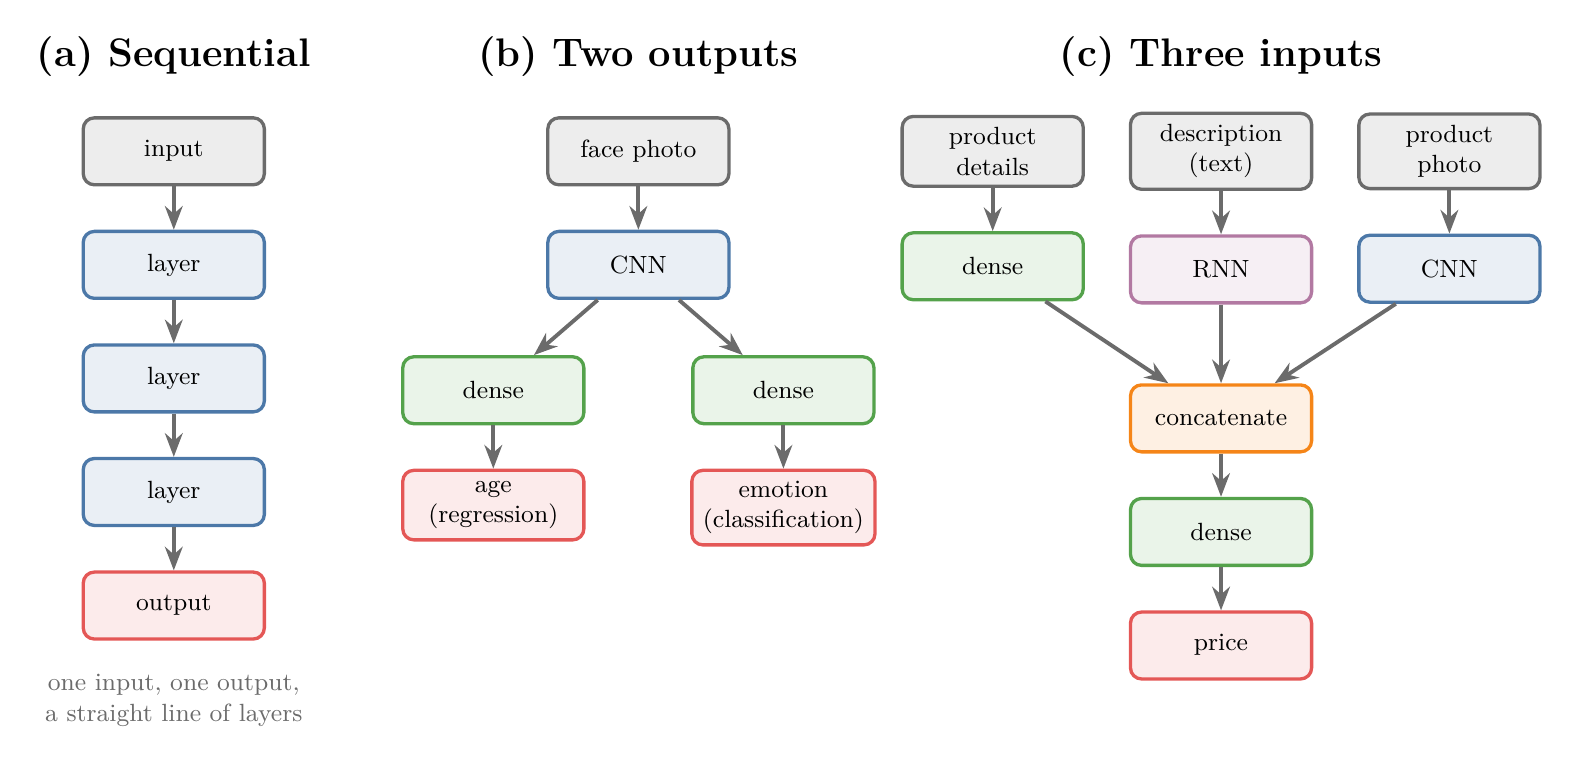
\begin{tikzpicture}[b/.style={box=#1, minimum width=2.3cm, minimum height=0.85cm, inner sep=4pt, font=\sffamily\small}, node distance=0.55cm]
  % (a) Sequential
  \begin{scope}
    \node[title] at (1.2, 1.2) {(a) Sequential};
    \node[b=cgrey] (i) at (1.2, 0) {input};
    \node[b=cblue, below=of i] (l1) {layer};
    \node[b=cblue, below=of l1] (l2) {layer};
    \node[b=cblue, below=of l2] (l3) {layer};
    \node[b=cred, below=of l3] (o) {output};
    \foreach \a/\c in {i/l1, l1/l2, l2/l3, l3/o} \draw[arrow] (\a) -- (\c);
    \node[note, below=0.3cm of o] {one input, one output,\\a straight line of layers};
  \end{scope}
  % (b) two outputs
  \begin{scope}[xshift=5.2cm]
    \node[title] at (1.9, 1.2) {(b) Two outputs};
    \node[b=cgrey] (f) at (1.9, 0) {face photo};
    \node[b=cblue, below=of f] (cnn) {CNN};
    \node[b=cgreen, below left=0.7cm and -0.5cm of cnn] (d1) {dense};
    \node[b=cgreen, below right=0.7cm and -0.5cm of cnn] (d2) {dense};
    \node[b=cred, below=of d1] (age) {age\\(regression)};
    \node[b=cred, below=of d2] (emo) {emotion\\(classification)};
    \draw[arrow] (f) -- (cnn); \draw[arrow] (cnn) -- (d1); \draw[arrow] (cnn) -- (d2);
    \draw[arrow] (d1) -- (age); \draw[arrow] (d2) -- (emo);
  \end{scope}
  % (c) three inputs
  \begin{scope}[xshift=11.6cm]
    \node[title] at (2.9, 1.2) {(c) Three inputs};
    \node[b=cgrey] (t) at (0, 0) {product\\details};
    \node[b=cgrey] (x) at (2.9, 0) {description\\(text)};
    \node[b=cgrey] (im) at (5.8, 0) {product\\photo};
    \node[b=cgreen, below=of t] (td) {dense};
    \node[b=cpurple, below=of x] (xr) {RNN};
    \node[b=cblue, below=of im] (ic) {CNN};
    \node[b=corange, below=1.0cm of xr] (cat) {concatenate};
    \node[b=cgreen, below=of cat] (dd) {dense};
    \node[b=cred, below=of dd] (price) {price};
    \draw[arrow] (t) -- (td); \draw[arrow] (x) -- (xr); \draw[arrow] (im) -- (ic);
    \draw[arrow] (td) -- (cat); \draw[arrow] (xr) -- (cat); \draw[arrow] (ic) -- (cat);
    \draw[arrow] (cat) -- (dd); \draw[arrow] (dd) -- (price);
  \end{scope}
\end{tikzpicture}
\end{document}
